\section{Delay Estimation}
\label{sec:03_delay}

To ascertain the direction of the sound source on one robot, the
delay of the signal from each channel to it's neighboring
next channel is the key information.
The implementation of the \ac{CC} from \cref{sec:02_cc} and the \ac{GCC-PHAT}
introduced in \cref{sec:02_gcc}, as well as the phase difference method
of \cref{sec:02_phase} will be presented shortly.

For all methods performed in frequency domain, the \ac{FFT} of the
signal is required. Hence the library NumPy for Python codes, known for it's high-level
mathematical functions also provides a module with fundamental
functions for the \ac{DFT}, \lstinline!numpy.fft.fft()! and
\lstinline!numpy.fft.ifft()! can be utilized.
In C++, the library \ac{FFTW} exists and delivers the same \ac{DFT} functions.
To estimate the delay between \lstinline!signal_0! and \lstinline!signal_1!,
both frames of the signals were Hann windowed in advance.
% -------------------------------------------------------------
\subsection*{Correlation}
\label{subsec:03_cc}

In Python, using the \ac{DFT} functions given by NumPy the \ac{CC} and \ac{GCC} calculation
can be implemented with little lines of code.
% Function \lstinline!correlation! of \cref{lst:03_cc} itemizes the steps to accomplish
\missing[]{text}
a correlation in Python with input signals \lstinline!x0! and \lstinline!x1!.
Determining the index of the maximal value of the correlation relative to the zero delay
index delivers the delay of \lstinline!x1! compared to \lstinline!x1! as the function
\lstinline!compute_delay! demonstrates.
% -------------------------------------------------------------
\subsection*{Subsample Delay}
\label{subsec:03_subsample}

Integer delays only offers resulting direction angles with low resolution.
To avoid this, the subsample shift estimation as in \cref{sec:02_subsampleShift}
is added to the delay estimation.

\subsection*{Phase Difference}
\label{subsec:03_phase}

There are two ways to determine the angle by phase difference
between two channels.
One can either look at the phase of a fixed frequency or set the frequency
dynamically.
For both, the signal must be divided into multiple frames.
The implementation for the fixed frequency case is straight forward.
From the result of the signal start detection, the frames
are set with an appropriate frame size and then transformed into
frequency domain.
As we know, the frequency of the whistle is between 2\si{\kilo\hertz}
and 4\si{\kilo\hertz}.
Thus, a suitable frequency in this range is chosen for analysis.
In the other case, the frame is chosen by doing a
frequency analysis.
For each channel frame in frequency domain after signal start,
the maximal absolute value and its belonging frequency is determined.
If this frequency is equal for all channels, these frames
are chosen.
\Cref{fig:03_maxFreq} shows that such frames exists for signals that
were transformed into frequency domain with a frame size of 256.
The frequency resolution changes with zero padding the signal prior
to the transformation.
\change[]{Finalize!}
% -------------------------------------------------------------
\begin{figure}[ht]
	\centering
		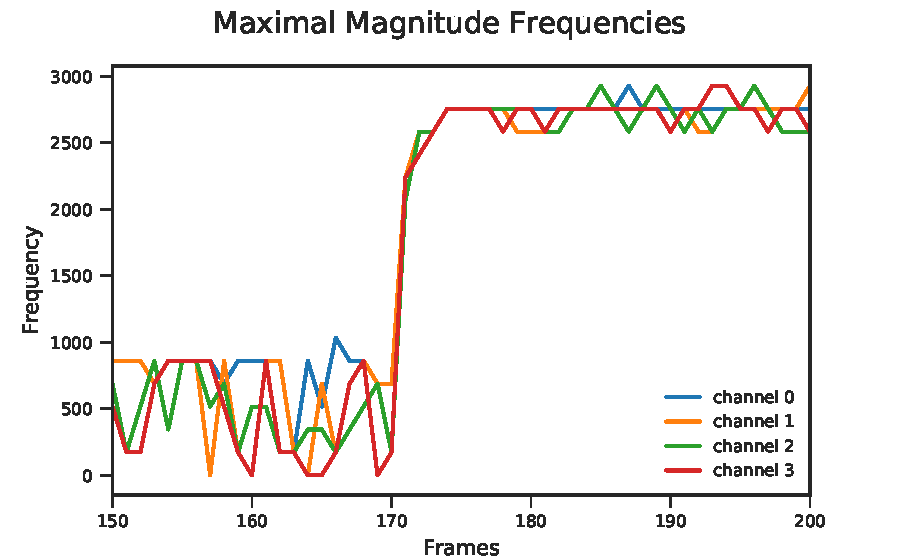
\includegraphics[]{figures/maxFreq}
	\caption{}
    \label{fig:03_maxFreq}
\end{figure}
% -------------------------------------------------------------

If the \ac{TDOA} is determined by phase difference, it must be ensured
that the maximal difference between two channels must not overflow $\pi$.
Meeting this condition, the signed difference is ascertainable.
As \cref{tab:03_maxFrequncies} presents, the distance between channel 0 and 1
is too large because its maximal frequency is not in whistle frequency range.
For this reason, the phase difference information between this pair is neglected.
% -------------------------------------------------------------
\btline{ht}{1.2}
\btab{|c|c|c|}
\hline
Channel Pairs & Absolute Distance [\si{\meter}] & Max. Frequency [\si{\hertz}]\\
\hline
0 and 1 & 0,116 & 1536,75\\
\hline
1 and 3 & 0,0533 & 3217,11\\
\hline
2 and 0 & 0,0533 & 3217,11\\
\hline
2 and 3 & 0.0618 & 2775,08\\
\hline
\etab
\et{Maximal feasible frequencies for unambiguous phase difference detection}{03_maxFrequncies}
% -------------------------------------------------------------

To facilitate the implementation, the phase difference is easily convertible into
delay samples $D_s$ with
\bal
	D_s = \frac{f_s \cdot \Delta \psi}{2 \pi \cdot f_c}.
\eal